\documentclass[11pt]{article}
\usepackage{fullpage}
\usepackage{graphicx}
\usepackage{amsmath}
\usepackage{url}
\usepackage{times,float}
%\usepackage{program}
\usepackage{subfigure}
%\usepackage{amsfonts}
%\usepackage{mathptm}

\textheight 50pc
\textwidth 38pc
\topmargin -3.0pc
\oddsidemargin 0pc
\evensidemargin -1pc
\marginparsep -1pc
\marginparwidth 0pc

\floatstyle{boxed}
\newfloat{algorithm}{thp}{loa}
\floatname{algorithm}{Algorithm}

\newcommand{\comment}[1]{\textit{\small {#1}}}
\newcommand{\cpp}{C\texttt{++}\ }
\newcommand{\tcl}{\textsc{Tcl\ }}
\newcommand{\ProtoMol}{\textsc{ProtoMol}}
\newcommand{\SamdII}{\textsc{Samd 2\ }}
\newcommand{\MOLLY}{\textsc{MOLLY\ }}

%\newcommand{\eqref}{\ref}

\newcommand{\tempstart}{\texttt{<}}
\newcommand{\tempend}{\texttt{>}}
\newcommand{\rij}{\mbox{r$_{ij}$}}
\newcommand{\rik}{\mbox{r$_{ik}$}}
\newcommand{\vrij}{\mbox{$\vec{r}_{ij}$}}
\newcommand{\Si}[1]{\mbox{Si$_{#1}$}}
\newcommand{\Vr}[1]{\mbox{$\vec{r}_{#1}$}}
\newcommand{\Vx}[1]{\mbox{$\vec{x}_{#1}$}}
\newcommand{\Vv}[1]{\mbox{$\vec{v}_{#1}$}}
\newcommand{\hatr}[1]{\mbox{$\hat{{r}_{#1}}$}}
\newcommand{\hatv}[1]{\mbox{$\hat{{v}_{#1}}$}}
\newcommand{\AbsVr}[1]{\mbox{$\left| \vec{r}_{#1} \right| $}}
\newcommand{\AbsVv}[1]{\mbox{$\left| \vec{v}_{#1} \right| $}}

\begin{document}
\thispagestyle{empty}

\title{
\begin{Large}
Hydrogen Group Decoupling For \MOLLY Integrators
\end{Large}
}
\author{Qun Ma \& Jes\'us Izaguirre}
\bigskip
\date{\today}
\maketitle

\parskip 0.3cm

%%%%%%%%%%%%%%%%%%%%%%%%%%%%%%%%%%%%%%%%%%%%%%%%%%%%%%%%%%%%%%%%%%%%%%%%%

\section{Introduction to multiple time stepping (MTS) integrators}
\subsection{Verlet-I/r-RESPA integrators}
Molecular dynamics for a classical
 unconstrained simulation requires the
 solution of Newton's equations of motion:
\begin{equation}
M\frac{\displaystyle {\mathrm d}^2}{\displaystyle {\mathrm d}t^2}{X}(t) = -\nabla U(X(t))
\label{eq:newton}
\end{equation}
where $M$ is a diagonal matrix of atomic masses, $x=X(t)$ are the atomic
trajectories, and the potential field $U$ is typically given by
\begin{eqnarray}
U &= &U^{\mathrm{bnd}}+U^{\mathrm{nonbnd}}, \\
U^{\mathrm{bnd}} & = &U^{\mathrm {bond}}+U^{\mathrm
{angle}}+U^{\mathrm{dihedral}}+U^{\mathrm{improper}}, \\ 
U^{\mathrm{nonbnd}} & = &U^{\mathrm{Lennard-Jones}}+U^{\mathrm{electrostatic}}.
\label{eq:potential}
\end{eqnarray}

The Verlet-I/r-RESPA multiple time stepping impulse method splits the
force into different components whose dynamics correspond to different
time scales, which are then represented as appropriately weighted
impulses (with weights determined by consistency). The impulse method
is
\begin{equation}
M\frac{\mathrm{d^{2}}}{\mathrm{d}t\mathrm{^{2}}}X=-\sum_{n^{\prime}=-\infty}^{\infty
}\delta t\ \mbox{\boldmath$\delta$}(t-n^{\prime}\Delta t)\nabla U^{\mathrm{fast}
}(X)-\sum_{n=-\infty}^{\infty}\Delta t\ \mbox{\boldmath$\delta$}(t-n\Delta
t)\nabla U^{\mathrm{slow}}(X) \label{eq:mts000}
\end{equation}
where the partitioning of{ }$U$\/\ into{ }$U^{\mathrm{fast}}$\/{\ }and{
}$U^{\mathrm{slow}}$\/{\ }is chosen so that an appropriate time step $\Delta
t$\/ for the slow part of the force is larger than a time step{ }$\delta t$
for the fast part.

Verlet-I/r-RESPA was proposed but not implemented by the authors
of~\cite{Grub89} and~\cite{GHWS91} and independently
discovered by the authors of~\cite{TuBM92}, who also
demonstrated its usefulness. It permits an increase to 4\thinspace fs
in the length of the longest time step $\Delta t.$ When the method was
introduced, it was predicted that there would occur resonances that
might induce instability if the frequency of the slow force impulse
coincides with a normal mode frequency of the system
\cite{GHWS91,BiSk93}. Resonance produces an oscillation in the positions
whose amplitude increases with time. More surprisingly, there is also
a problem for long time steps just smaller than half the period of the
fastest normal mode \cite{GaSS98b,BaSc98b}. There is also empirical
evidence that time steps of 5\thinspace fs or greater are not possible
with this method \cite{BiSS97}.


\subsection{\MOLLY integrators}
\MOLLY is a family of integrators~\cite{GaSS98b} that counteracts the
instabilities present 
in the multiple time stepping Verlet-I/r-RESPA integrator. This is
accomplished by perturbing the potential using time averaged positions 
\begin{equation}
U^{{\rm slow}}(x)\rightarrow U^{{\rm slow}}({\mathcal{A}}(x)),
\end{equation}
with the force defined as a gradient of this averaged potential, 
\begin{equation}
-\nabla U^{{\rm slow}}(x)\rightarrow -{\mathcal A}_{x}(x)^{{\rm T}}\nabla U^{
{\rm slow}}({\mathcal A}(x)).
\end{equation}

This perturbation is supposed to compensate for finite $\Delta t$ artifacts.
Perturbing the potential rather than the force ensures that the numerical
integrator is symplectic \cite{SaCa94}. The force used by \MOLLY is
the gradient 
of the perturbed potential \cite{IzRS99}. \MOLLY can be seen as a filter that
eliminates components of the slow force impulse in the directions of the
fast forces, and thus improves the stability of Verlet-I/r-RESPA. Different
averaging functions give rise to \MOLLY integrators with different stability
and accuracy properties. For instance, an averaging based on spectral
methods allows very precise filtering, but due to the diagonalizing of a
Hessian, is computationally expensive. Reference \cite{GaSS98b} suggests
using an averaging function ${\mathcal A}(x)$ that takes into account
the motion 
induced by some of the fast forces (those that are the gradient of a simpler
energy, $U^{{\rm fastest}}).$ This reduced system is then integrated over a
short time span (typically for an interval of order $\Delta t$) using weight
functions with local support in time (e.g. B-splines). The main
computational expense of these B-spline averagings is the computation of
force Hessian-vector products (needed to generate the filter ${\mathcal A}
_{x}(x)).$ These averagings overcome the 5\thinspace fs barrier and their
effectiveness is related to the extensiveness of the time averaging \cite
{SkIz98}.


\subsection{B-spline averagings\label{se:b-spline}}

It is possible to use time averagings that consist of numerically integrating
an auxiliary, reduced problem:
\begin{equation}
\mathcal{A}(x)=\frac{1}{\Delta t}\int_{0}^{\infty}\phi\left(  \frac{t}{\Delta
t}\right)  \tilde{X}(t)dt \label{eq:weightave}
\end{equation}
where $\phi\left(  \frac{t}{\Delta t}\right)  $
\index{01w0phifun@$\phi(s)\mathcal{\qquad}$\ Weight function of compact
support} is a weight function, and $\tilde{X}(t)$
\index{02X2XTILDE@$\tilde{X}\mathcal{\qquad}$\ Positions for auxiliary
problem} solves an \emph{auxiliary} problem
	\begin{equation}
M\frac{\mathrm{d}^{2}}{\mathrm{d}t^{2}}\tilde{X}=F^{\mathrm{reduced}}
(\tilde{X}),\quad\tilde{X}(0)=x,\quad\frac{\mathrm{d}}{\mathrm{d}t}\tilde
{X}(0)=0. \label{eq:reducedflow}
\end{equation}

This approach is computationally feasible if the weight functions $\phi$ have
compact support in time. The paper~\cite{GaSS98b} suggests using
B-spline weight 
functions, which are non-zero over a short interval. The effectiveness of the
averagings induced by these weight functions is directly related to the
extensiveness of the time averaging.

Several B-spline weight functions that were tested are shown next:

\begin{description}
\item \textbf{ShortAverage}
\begin{equation}
\phi(s) = \begin{cases}
	0, & \quad s < 0,	\\
	2, & \quad 0 \leq s < \frac{1}{2},\\
	1, & \quad s = \frac{1}{2}, \\
	0, & \quad s > \frac{1}{2}.
	\end{cases}
\label{eq:bspline00}
\end{equation}

\item \textbf{LongAverage}
\begin{equation}
\phi(s) = \begin{cases}
	0, & \quad s < 0,	\\
	1, & \quad 0 \leq s < 1, \\
	\frac{1}{2},& \quad s = 1,\\
	0, & \quad s > 1.
	\end{cases}
\label{eq:bspline0}
\end{equation}

\item \textbf{LongLinearAverage}
\begin{equation}
\phi(s) = \begin{cases}
	0, & \quad s < 0,	\\
	1 - \frac{1}{2} s, & \quad 0\leq s\leq2,\\
	0, & \quad s > 2.
	\end{cases}
\label{eq:bspline1}
\end{equation}

\item \textbf{LongQuadraticAverage}
\begin{equation}
\phi(s) = \begin{cases}
	0, & \quad s < 0,	\\
	\frac{1}{4}(3-s^{2}), & \quad 0 \leq s < 1,\\
	\frac{1}{8}(3-s)^{2}, & \quad 1 \leq s \leq 3,\\
	0, & \quad s > 3.
	\end{cases}
\label{eq:bspline2}
\end{equation}
\end{description}
The last three are plotted in Fig.~\ref{fig:bspline}.
\begin{figure}[ptb]
\begin{center}
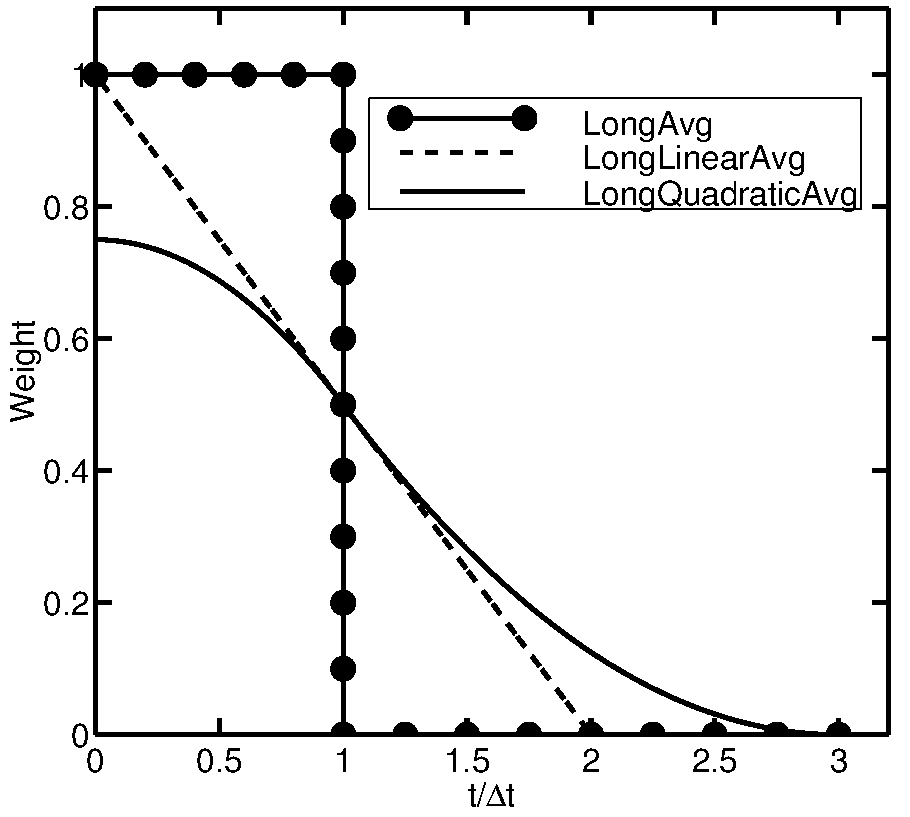
\includegraphics[
height=3in
%height=5.5037in,
%width=6.1367in
]
{figs/bspline.pdf}
\caption{Weight vs. $t/\Delta t$ for first three B-spline filters.}
\label{fig:bspline}
\end{center}
\end{figure}

%In the frequency domain, using more extensive averagings is equivalent to
%using higher powers of sinusoidal filters. 
%This can be seen by applying
%standard Fourier transforms to Eqs.~\eqref{eq:bspline00}--\eqref{eq:bspline2}
%(see tables in~\cite[pp.~18,19]{EMOT54}), for which the formulas become:


%\begin{description}
%\item \textbf{ShortAverage}
%\begin{equation}
%\Phi\left(  \omega\right)  =\frac{\sin\frac{\Delta t}{2}\omega}{\frac{\Delta
%t}{2}\omega}. \label{eq:freq00}
%\end{equation}

%\item \textbf{LongAverage}
%\begin{equation}
%\Phi\left(  \omega\right)  =\frac{\sin\Delta t\omega}{\Delta t\omega}.
%\label{eq:freq0}
%\end{equation}

%\item \textbf{LongLinearAverage}
%\begin{equation}
%\Phi\left(  \omega\right)  =\left(  \frac{\sin\Delta t\omega}{\Delta t\omega
%}\right)  ^{2}. \label{eq:freq1}
%\end{equation}

%\item \textbf{LongQuadraticAverage}
%\begin{equation}
%\Phi\left(  \omega\right)  =\left(  \frac{\sin\Delta t\omega}{\Delta t\omega
%}\right)  ^{3}. \label{eq:freq2}
%\end{equation}
%\end{description}

%\begin{figure}[ptb]
%\begin{center}
%\includegraphics[
%height=3in
%height=5.6066in,
%width=6.0226in
%]
%{figs/mollyfilter.pdf}
%\caption{Effect of higher powers of a simple sinusoidal filter on high
%5 frequencies. These filters are Fourier transforms of the B-spline averagings
%used by MOLLY. Higher powers damp high frequencies more effectively, and
%correspond to more extensive time averagings.}
%\label{fig:frequencymolly}
%\end{center}
%\end{figure}

In the frequency domain, using more extensive averagings is equivalent to
using higher powers of sinusoidal filters. 
Higher powers of such simple filters are better because the high frequencies
of $F^{\mathrm{slow}}$ are more effectively damped.
%(cf. Figure~\ref{fig:frequencymolly}).
Interestingly, the accuracy of B-spline MOLLY is not reduced by
increasing the strength of $F^{\mathrm{reduced}}$ whereas that of
Verlet-I/r-RESPA is (for the latter the error term is increased from
$O(\Delta t^{2})$ to $O(\Delta t)$ for faster $F^{\mathrm{reduced}}).$

The previous implementation of B-spline \MOLLY integrators 
uses Hessian matrices (required for the mollification of
the slow force impulse) generated by automatic differentiation tools for C++
developed at Argonne National Labs~\cite{ADOL-C}. 
Although it is quite beneficial to use
this tool to do these computations in the proof-of-concept stage, it can
not be used to large systems because of efficiency. As a result, in
order to make B-Spline \MOLLY integrator part of our production code,
\ProtoMol, we have to compute the Hessian matrices
directly. Fortunately, we already had derived and verified the
analytical expressions of the Hessian matrices \cite{MaIz01}.
The coding of $\mathcal{A}
(x)$ and $\mathcal{A}_{x}(x),$ now, can be done by hand in a systematic
manner. First the calculation of $\mathcal{A}(x)$ is coded, and then this is
differentiated applying the chain rule with respect to each of the components
of $x$ to yield code for $\mathcal{A}_{x}(x)$. As an example suppose that the
leapfrog method with time step $\delta t$ is coded for the calculation of
$\mathcal{A}(x)$. This is then differentiated to obtain $\mathcal{A}_{x}(x)$.
The result is the following code for calculating $\mathcal{A}(x)$ and
$\mathcal{A}_{x}(x)$:

Initialization is given by
\begin{equation}
\begin{array}
[c]{cc}
X:=x, & X_{x}:=I,\\
P:=0, & P_{x}:=0,\\
B:=0, & B_{x}:=0,
\end{array}
\end{equation}
and step by step integration by
\begin{equation}
\begin{array}
[c]{ll}
P:=P+\frac{1}{2}\delta tF^{\mathrm{reduced}}(X), & P_{x}:=P_{x}+\frac{1}
{2}\delta tF_{x}^{\mathrm{reduced}}(X)X_{x},\\
B:=B+\frac{1}{2}\delta tX, & B_{x}:=B_{x}+\frac{1}{2}\delta tX_{x},\\
X:=X+\delta tM^{-1}P, & X_{x}:=X_{x}+\delta tM^{-1}P_{x},\\
B:=B+\frac{1}{2}\delta tX, & B_{x}:=B_{x}+\frac{1}{2}\delta tX_{x},\\
P:=P+\frac{1}{2}\delta tF^{\mathrm{reduced}}(X), & P_{x}:=P_{x}+\frac{1}
{2}\delta tF_{x}^{\mathrm{reduced}}(X)X_{x}.
\end{array}
\end{equation}
The value $(1/\Delta t)B$ is used for $\mathcal{A}(x)$ and $(1/\Delta t)B_{x}$
for $\mathcal{A}_{x}(x)$. We continue the above integration until we
reach a value of $t$ such that $\phi(t/\Delta t)$ is zero at this
value and remains zero for larger values of $t.$ For example, for
ShortAverage this means getting the value $B(\frac{\Delta t}{2} +
\delta t)$ because $\phi(t/\Delta t)$ vanishes only for
$t>\frac{1}{2}.$ Equivalently, for the purpose of programming, we can
define $\phi(\frac{1}{2})$ to be $1$ rather than $\frac{1}{2}$ and stop 
at $t = \frac{\Delta t}{2}.$  In practice, one would like to choose
$\delta t = \frac{\Delta t}{2}.$ If such is the case, and
if ShortAverage is used, then one gets a handy equation for computing 
$\mathcal{A}_{x}(x):$
\begin{equation}
\label{eqn:ax}
\mathcal{A}_{x}(x) = I + \frac{1}{16} \Delta t^2 M^{-1} F_x(x)
\end{equation}
where $F_x = - U^\mathrm{reduced}_{xx}(x).$


\section{Expriments on water systems using B-spline MOLLY integrator}
Water systems are easy to experiment with since all the water
molecules are separate from each other. Figure \ref{fig:water} shows
one water molecule.
\begin{figure}[hbt]
\centerline{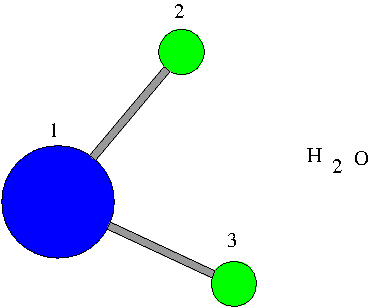
\includegraphics[width=2.0in]{figs/water.pdf}}
\caption{Ball stick representation of a water molecule}
\label{fig:water}
\end{figure}

In order to mollify the slow force impulses acted on each atom, and if 
only bond and angle energies are included in the reduced system, we
have to assemble the bond Hessians and angle Hessian to form a
complete Hessian for one single molecule. Suppose the
Hessian matrices of bond energy for atoms $1$ and $2$, and $1$ and
$3$, {\it i.e.,} $H^{\mathrm{bd12}}$ and $H^{\mathrm{bd13}}$, and the
angle Hessian matrix for atoms $1$ $2$ and $3$, {\it i.e.,}
$H^{\mathrm{a123}}$ are given as follows:
\begin{eqnarray}
H^{\mathrm{bd12}} &=& \left[
\begin{tabular} {cc}
$H^{\mathrm{bd12}}_{11}$ & $H^{\mathrm{bd12}}_{12}$ \\
$H^{\mathrm{bd12}}_{21}$ & $H^{\mathrm{bd12}}_{22}$ 
\end{tabular}
\right]\\
H^{\mathrm{bd13}} &=& \left[
\begin{tabular} {cc}
$H^{\mathrm{bd13}}_{11}$ & $H^{\mathrm{bd13}}_{12}$ \\
$H^{\mathrm{bd13}}_{21}$ & $H^{\mathrm{bd13}}_{22}$ 
\end{tabular}
\right] \\
H^{\mathrm{a123}} &=& \left[
\begin{tabular} {ccc}
$H^{\mathrm{a123}}_{11}$ & $H^{\mathrm{a123}}_{12}$ &
$H^{\mathrm{a123}}_{13}$ \\
$H^{\mathrm{a123}}_{21}$ & $H^{\mathrm{a123}}_{22}$ & 
$H^{\mathrm{a123}}_{23}$ \\
$H^{\mathrm{a123}}_{31}$ & $H^{\mathrm{a123}}_{32}$ & $H^{\mathrm{a123}}_{33}$ 
\end{tabular}
\right].
\end{eqnarray}
Then the assembled Hessian matrix for this whole molecule is as follows:
\begin{equation}
H^{\mathrm{total}} = \left[
\begin{tabular} {ccc}
$H^{\mathrm{a123}}_{11}+H^{\mathrm{bd12}}_{11}+
H^{\mathrm{bd13}}_{11}$ 
& $H^{\mathrm{a123}}_{12}+H^{\mathrm{bd12}}_{12}$ &
$H^{\mathrm{a123}}_{13}+H^{\mathrm{bd13}}_{12}$  \\ 
$H^{\mathrm{a123}}_{21}+H^{\mathrm{bd12}}_{21}$   
& $H^{\mathrm{a123}}_{22}+H^{\mathrm{bd12}}_{22}$ &  
$H^{\mathrm{a123}}_{23}$  \\ 
$H^{\mathrm{a123}}_{31}+H^{\mathrm{bd13}}_{21}$  & $H^{\mathrm{a123}}_{32}$ & $H^{\mathrm{a123}}_{33}+H^{\mathrm{bd13}}_{22}$
\end{tabular}
\right].
\end{equation}
Substitute $F_x(x)$ in
Equation~(\ref{eqn:ax}) with $-H^{\mathrm{total}},$ one gets the the
filter $\mathcal{A}_{x}(x).$

Figure \ref{fig:water_benchmark} shows the percent relative variation
in energy $\Delta E (\mathrm{kcal}\, \mathrm{mol}^{-1}\,
\mathrm{K}^{-1})$ vs $\Delta t (\mathrm{fs})$ using ShortAverage
B-spline \MOLLY integrator. 

\begin{figure}[hbt]
%\centerline{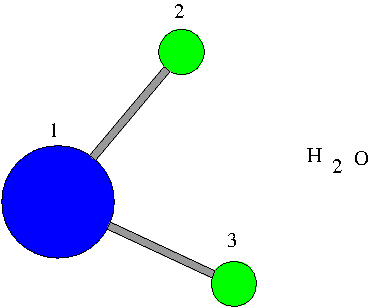
\includegraphics[width=20.in]{figs/water.pdf}}
\caption{Water benchmark results.}
\label{fig:water_benchmark}
\end{figure}

\section{Hydrogen group decoupling for biomolecules}
The early efforts in B-spline \MOLLY integrators, however,
were mainly on  water systems. In order 
to extend the use of this kind of integrators to biomolecular
systems, {\it e.g.} proteins and DNAs, we need to do some extra work,
namely, reordering of the lists for bonds and angles to form hydrogen
groups (HG) so that we could perform mollification correctly. 

A hydrogen group is a group of hydrogen atoms and a heavy atom (be it
an oxygen, carbon, or sulfur) bonded
together by linear bonds, angular bonds, dihedral and improper bonds. 
When we have this data structure and correct ordering, we can then
mollify the force acted on one atom completely in one step.

Hydrogen group decoupling (HGD), although it is a somewhat {\it ad hoc}
approach,  helps to capture the most important
destablizing factors in MTS integrators since the natural frequency of 
the hydrogen-heavy atom interaction is highest amongst other natural
frequencies in the simulated system. HGD greatly simplifies
mollification process which now can be done relatively efficiently. 
The counterpart of this technique is to include all possible fast
interactions among all atoms and thus to have a completely general
sparse mollification matrix, $\mathcal{A}_{x}(x).$ The tradeoff
between these two approaches is apparently efficiency and
accuracy. We will see if HGD is accurate enough with more experiments.


\subsection{The algorithms for hydrogen group decoupling}
Figure \ref{fig:met} shows the structure of an amino acid,
Methionine, in which the HGs are circled with dotted lines. 
Let's assume that the atoms were numbered as shown in the
figure in the input file. Our goal is to sort the bond pairs and angle
triplets to get HGs of $(1,2,3)$, $(4,6,7)$,$(8,9,10,11)$ and thus get a
sorted bond list and a sorted angle list.
\begin{figure}[hbt]
\centering

\subfigure[Original numbering]{
\label{fig:met}
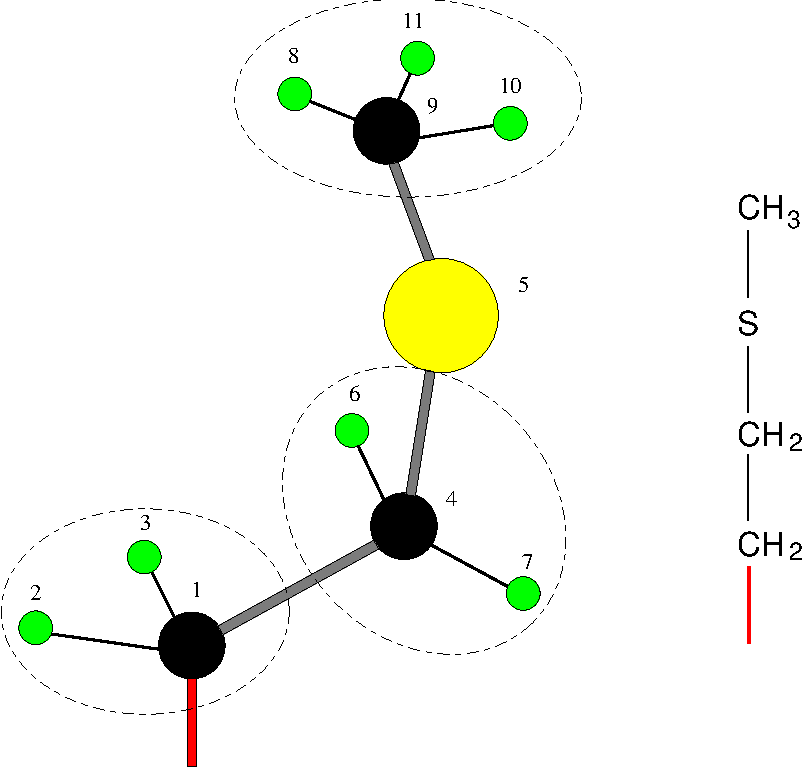
\includegraphics[width=200pt]{figs/met.pdf}}
\subfigure[Modified numbering]{
\label{fig:met2}
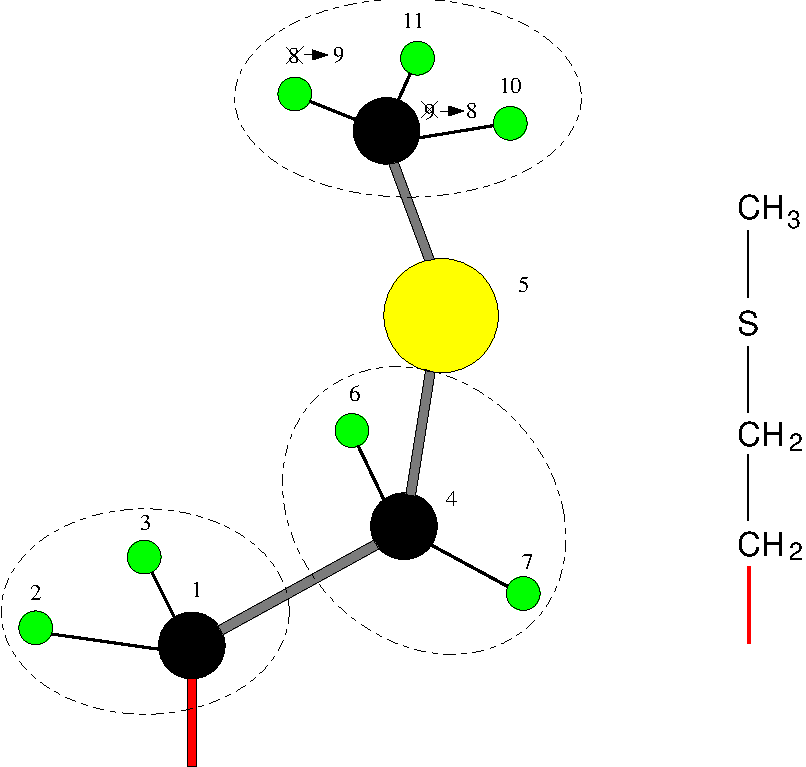
\includegraphics[width=200pt]{figs/met2.pdf}}
\caption{Ball stick representation of Methionine with original and
modified numbering schemes}
\end{figure}

The following algorithms describes a how to get the HGs and sort the
bonds and angles.

\begin{enumerate}
\label{HACF}
\item Heavy-Atom-Come-First: All heavy atoms should be numbered
smaller than all the hydrogen atoms bonded to them. Even better if a
HG is completed before another HG. This makes a HG contiguous in memory.
A re-numbered system is shown in Figure \ref{fig:met2} in which atoms
$8$ and $9$ are swapped. Remember that all the attributes associated
with these swapped atoms should also swap. For any system, this
re-numbering procedure would only take place in the beginning of
simulation and done in Front-End. Question: What about IMD? One idea
is to keep permutation vector in the beginning. 
\begin{algorithm}
\caption{ Heavy-Atom-Come-First.}
\begin{verbatim}
begin:	
   read in PDB file of biomolecules
   for each atom 
      if the atom is not hydrogen
          put the atom in a queue  

   for each heavy atom in the queue
      for each atom connected to the heavy atom
          if its number is bigger than that of the heavy atom
             renumber the heavy atom and the hydrogen atom such 
             that the heavy atom number is smaller than all other 
             hydrogen atoms
end:
\end{verbatim}
\end{algorithm}


\item Sort-Bonds: Go through all bonds and ensure that smaller numbers 
appear before bigger ones. First compare numbers in each bond, swap
the numbers if bigger one comes before smaller one. After this, sort
the list according to first numbers in each pair. 
\begin{verbatim}
       2 -- 1          1 -- 2          1 -- 2
       1 -- 3          1 -- 3          1 -- 3
       6 -- 4          4 -- 6          1 -- 4
       1 -- 4          1 -- 4          4 -- 6
       4 -- 7   ===>   4 -- 7   ===>   4 -- 7
       4 -- 5          4 -- 5          4 -- 5
       5 -- 8          5 -- 8          5 -- 8
       9 -- 8          8 -- 9          8 -- 9
      11 -- 8          8 -- 11         8 -- 11
       8 -- 10         8 -- 10         8 -- 10
\end{verbatim}

\item Heavy-Atom-List (HAL): Go through all atoms, if $atom.name!='H*'$,
then push back to HAL. HAL should have members of heavy atom number,
and the number of bonds associated with this heavy atom. As a result
of this step, the HAL will be as follows:
\begin{verbatim}
      number     size
      1          0
      4          0
      5          0
      8          0
\end{verbatim}

\item Bonds-to-Hydrogen: Go through HAL. For each heavy atom, find all 
bonds in which it is involved. If the other atom is a hydrogen,
push back Bonds-To-Hydrogen, and increment size. As a result, the HAL
changes to the following:
\begin{verbatim}
      number     size
      1          2
      4          2
      5          0
      8          3
\end{verbatim}
And the sorted bonds-to-hydrogen is as follows:
\begin{verbatim}
      1 -- 2
      1 -- 3
      4 -- 6
      4 -- 7
      8 -- 9
      8 -- 11
      8 -- 10
\end{verbatim}

\item Remove-Non-HG-Angles: Go through angles, remove non-HG angles so
that only HG angles are left.

\item Sort-Angles: Go through angles, ensure that smallest atom number 
appear first.

The above two steps are shown as follows:
\begin{verbatim}
      2 - 1 - 3        2 - 1 - 3         1 - 2  - 3
      1 - 4 - 6        6 - 4 - 7         4 - 6  - 7   
      6 - 4 - 1  ===>  8 - 9 - 10  ===>  8 - 9  - 10
      1 - 4 - 5        9 - 8 - 11        8 - 9  - 11
      6 - 4 - 7       10 - 8 - 11        8 - 10 - 11
      6 - 4 - 5 
      7 - 4 - 5 
      5 - 8 - 10
      5 - 8 - 11
      5 - 9 - 8 
      4 - 5 - 8 
      8 - 9 - 10
      9 - 8 - 11
     10 - 8 - 11
\end{verbatim}
\end{enumerate}

\subsection{Challenges of including H-bonds in mollification process}
When only localized interactions are considered in the mollification
process for B-spline integrator, HGD most likely is going to work
well. What if H-bond is to be considered in the mollification process, 
{\it i.e.,} taking into account H-bond interaction when
$\mathcal{A}(x)$ is computed? Since H-bond is not localized
interaction that often times forms and disappears in a non-predictable
manner, we will not be able to compute $\mathcal{A}_{x}(x)$ as easy as 
we do before. How to maintain a list of active H-bonds, and how to
compute $\mathcal{A}_{x}(x)$ remain open questions. 

\bibliographystyle{abbrv}
\bibliography{lcls}

\end{document}



